% pygeek2026-en.tex
% PyGeek 2026 submission — English short paper (faithful translation of pygeek2026-ko.tex).
% Content transcribed verbatim from docs/research/paper-ko.md; this file
% is the typesetting layer only (see repo CLAUDE.md / task instructions).
% 구성은 지도교수 피드백(2026-08-08)에 따른 4절 체계:
%   1. 서론 / 2. 제안 방법(2.1~2.3) / 3. 성능평가(3.1~3.2) / 4. 결론
% 3쪽 압축판: 요인 분해 그림 삭제 → 표 1(실험 조건 구성)로 대체, 결과 표 12행→8행 축약,
%   구조도 그림 한 줄 노드 재제작(높이 -40%), 표 2와 중복되는 본문 통계 서술 제거.

\documentclass[10pt,a4paper,twocolumn]{article}

% ---------- fonts ----------
\usepackage{xetexko}
\latinparens            % ASCII 괄호·대괄호를 한글 글꼴이 아닌 본문(Times) 글꼴로 — 템플릿 표기와 일치
\setmainfont{Times New Roman}
\setmainhangulfont{Nanum Myeongjo}   % 템플릿의 바탕체(BatangChe) 미설치 → 동일 계열 명조체, 진짜 Bold 보유

% ---------- page geometry ----------
\usepackage[a4paper,left=1.78cm,right=1.78cm,top=1.78cm,bottom=1.78cm,%
            headheight=22pt,headsep=8pt,footskip=16pt,columnsep=1.27cm]{geometry}  % 수치는 PyGeek 공식 DOCX 템플릿의 pgMar/cols에서 추출

% ---------- misc packages ----------
\usepackage{fancyhdr}
\usepackage{graphicx}
\usepackage{amsmath}
\usepackage{unicode-math}
\setmathfont{STIX Two Math}   % Times 호환 수식 글꼴 (템플릿 본문 Times와 정합)
\usepackage{booktabs}
\usepackage{array}
\usepackage{url}
\urlstyle{same}   % URL·DOI도 본문 글꼴(Times)로 — 템플릿 참고문헌 표기와 일치
\Urlmuskip=0mu plus 1mu\relax          % 참고문헌 URL이 줄 어디서든 자연스럽게 끊기도록
\def\UrlBreaks{\do\/\do\-\do\.\do\:\do\_\do\?\do\=\do\&\do\a\do\b\do\c\do\d\do\e\do\f\do\g\do\h\do\i\do\j\do\k\do\l\do\m\do\n\do\o\do\p\do\q\do\r\do\s\do\t\do\u\do\v\do\w\do\x\do\y\do\z\do\0\do\1\do\2\do\3\do\4\do\5\do\6\do\7\do\8\do\9}   % URL·DOI도 본문 글꼴(Times)로 — 템플릿 참고문헌 표기와 일치
\usepackage{setspace}
\usepackage{textcomp}

\clubpenalty=10000\widowpenalty=10000   % 제목 직후 한 줄 고아·과부 줄 방지
\tolerance=1000
\emergencystretch=3em

% 두 폭 그림(figure*)이 페이지 상단에 자리 잡도록 허용
\renewcommand{\dbltopfraction}{0.95}
\renewcommand{\dblfloatpagefraction}{0.7}
\renewcommand{\topfraction}{0.95}
\renewcommand{\textfraction}{0.05}
\setcounter{dbltopnumber}{2}

% ---------- body typography: 10pt / 1.15 spacing / justified (default) ----------
\setstretch{1.15}
\setlength{\parindent}{0pt}
\setlength{\parskip}{1.2pt}

% ---------- running header / footer ----------
\pagestyle{fancy}
\fancyhf{}
\renewcommand{\headrulewidth}{0.6pt}
\renewcommand{\footrulewidth}{0pt}
\fancyhead[R]{\fontsize{10}{12}\selectfont 2026 International Conference on PyGeek (PyGeek 2026)}
\fancyfoot[R]{\thepage}

\fancypagestyle{firstpage}{%
  \fancyhf{}
  \fancyhead[L]{\fontsize{10}{12}\selectfont\parbox[b]{8cm}{2026 International Conference on PyGeek (PyGeek 2026)\\[1pt] Vol. xx, 2026}}
  \fancyhead[R]{\fontsize{10}{12}\selectfont ISSN (Online): 0000-0000}
  \renewcommand{\headrulewidth}{0.6pt}
  \fancyfoot[R]{\thepage}
}

% ---------- section heading macros (manual numbering, matches source text) ----------
\newcommand{\pgsec}[1]{\par\vspace{5pt}{\bfseries\fontsize{12}{14}\selectfont #1}\par\nobreak\vspace{2pt}\nobreak}
\newcommand{\pgsubsec}[1]{\par\vspace{4pt}{\bfseries\fontsize{12}{14}\selectfont #1}\par\nobreak\vspace{1pt}\nobreak}
\newcommand{\pgspecial}[1]{\par\vspace{5pt}\begin{center}{\bfseries\fontsize{12}{14}\selectfont #1}\end{center}\vspace{2pt}}

\begin{document}
\thispagestyle{firstpage}

% ======================================================================
% Full-width title block + bilingual abstracts (single column, first page)
% ======================================================================
\twocolumn[
  \begin{center}
    \setstretch{1.0}
        {\fontsize{16}{20}\selectfont\bfseries A Factor Decomposition Method for Separating Store Substitution and Embedding Placement Effects in Vector Database Migration}\par
  \end{center}
  \vspace{5pt}
  \noindent\rule{\linewidth}{0.6pt}\par
  \vspace{3pt}
  {\bfseries\fontsize{12}{14}\selectfont Abstract}\par
  \vspace{3pt}
  {\fontsize{8}{9.6}\selectfont
  When the vector layer of a retrieval-augmented generation (RAG) system is migrated to a different database, the effect is usually assessed by an end-to-end comparison of the system before and after the migration. That comparison, however, blends into a single measurement two changes that are independent yet occur together in practice, namely substituting the store engine and relocating where the embedding is computed, which makes it impossible to tell which factor caused the change. This paper proposes a method that introduces a bridge condition, in which the target store is loaded with the embeddings the source system has already produced, so that one comparison in which the two factors are entangled is split into two comparisons that each differ in one factor only. The bridge condition requires no re-embedding, so it is inexpensive and leaves the running service untouched. Applied to a Korean product-review RAG service in production (1,347 chunks, 43 queries), no change in retrieval quality was detected for the store substitution (top-10 Jaccard 0.971, relevance difference $-$0.042, $p = 0.52$), whereas relocating the embedding into the database produced a significant, medium-sized effect ($p = 0.003$, Cohen's $d_z = 0.47$). Virtually all of the observed change therefore originates from the embedding placement factor. The method does not judge the superiority of any particular product and applies to migrations to converged databases in general.
  \par}
  \vspace{4pt}
  {\bfseries\fontsize{9}{11}\selectfont Keywords: }{\fontsize{8}{9.6}\selectfont Retrieval-Augmented Generation, Vector Database, In-Database Embedding, Migration, Factor Decomposition}\par
  \vspace{4pt}
  \noindent\rule{\linewidth}{0.6pt}\par
  \vspace{6pt}
]

% ======================================================================
% 1. Introduction
% ======================================================================
\pgsec{1. Introduction}

A retrieval-augmented generation (RAG) system consists of an embedding model that turns queries and documents into vectors, a store that indexes and searches those vectors, and a language model that generates an answer grounded in the retrieved results [1], [2]. Among these, the component changed most often after deployment is the vector layer. A representative path leads from a general-purpose relational database with a vector extension to a converged database that has a vector type and an inference runtime inside it, that is, one in which the database itself performs the embedding computation.

The effect of such a migration is usually assessed by an end-to-end comparison that weighs the whole system before and after the change at once. In this comparison, however, two factors change at the same time. The first is the store, that is, the engine that holds the vectors and the indexing method it uses. The second is the placement, that is, whether the embedding is computed by an external service or by an inference runtime inside the database. When a migration is motivated by governance, moving the embedding inside as well is the preferred configuration, and a database that hosts a model limits the size of the model file. This is why the two factors change together in practice.

% Figures 1 & 2 (system architectures, section 2.1)
\begin{figure*}[t]
\centering
\begin{minipage}[t]{0.45\textwidth}
  \centering
  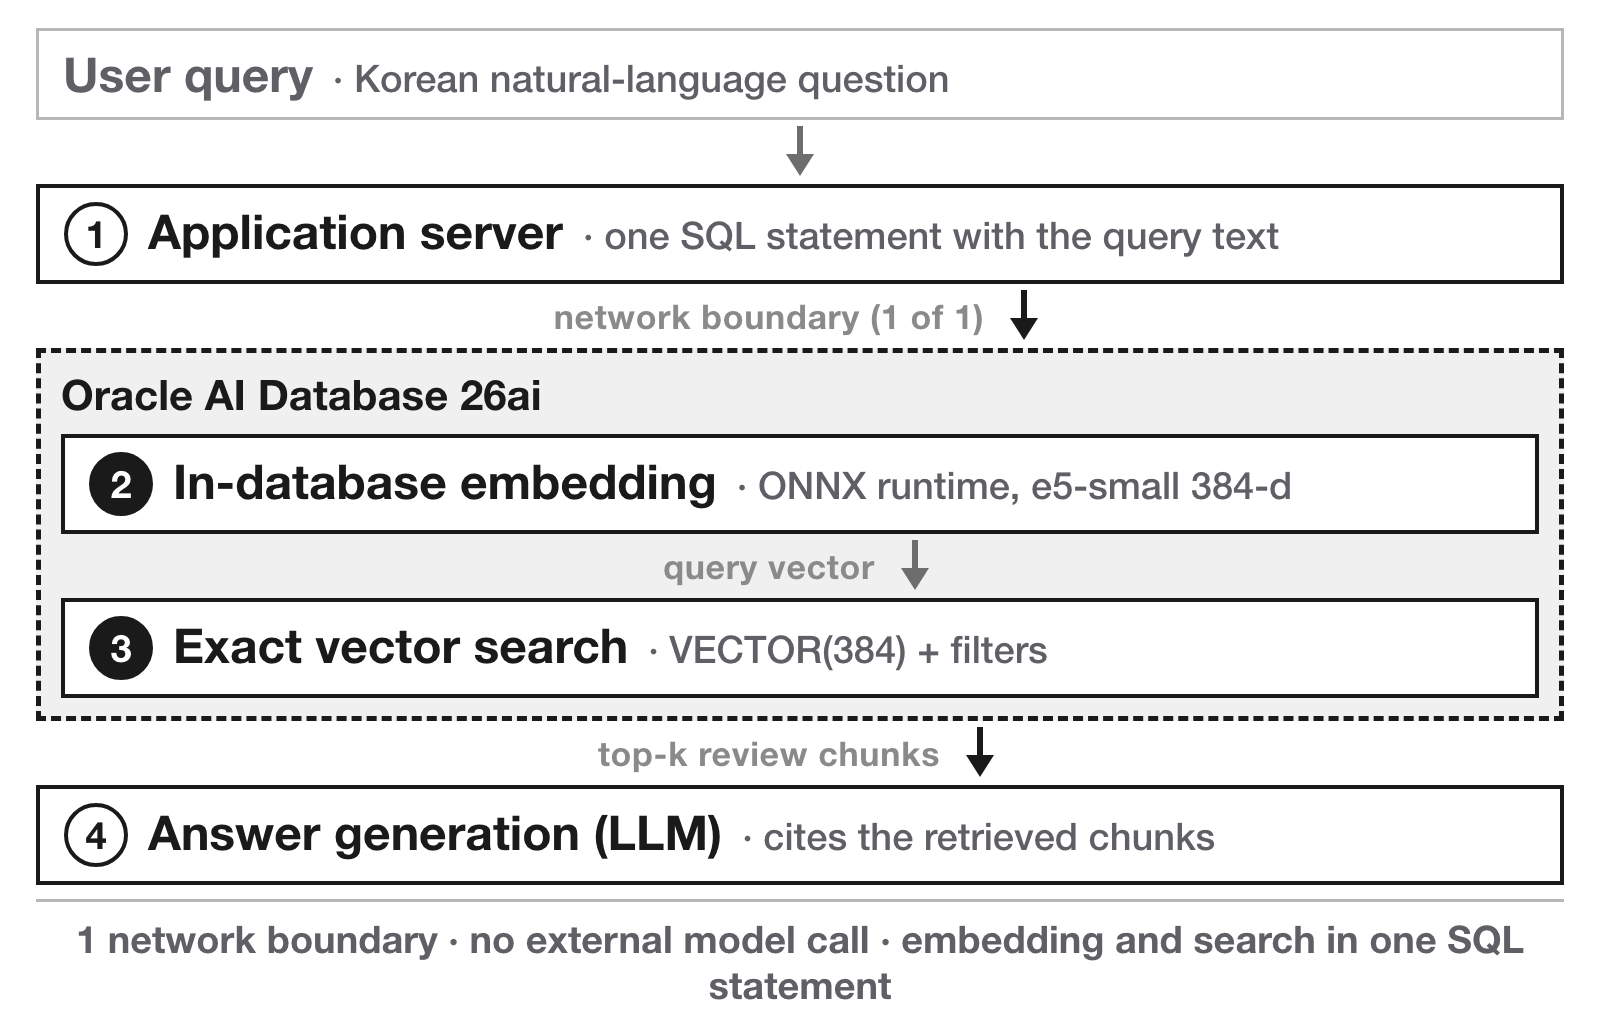
\includegraphics[width=\linewidth]{../../figures/paper-fig1-arch-oracle.png}\par
  \vspace{5pt}
  {\fontsize{8}{9.6}\selectfont Fig. 1. Oracle-based system architecture}
\end{minipage}\hfill
\begin{minipage}[t]{0.45\textwidth}
  \centering
  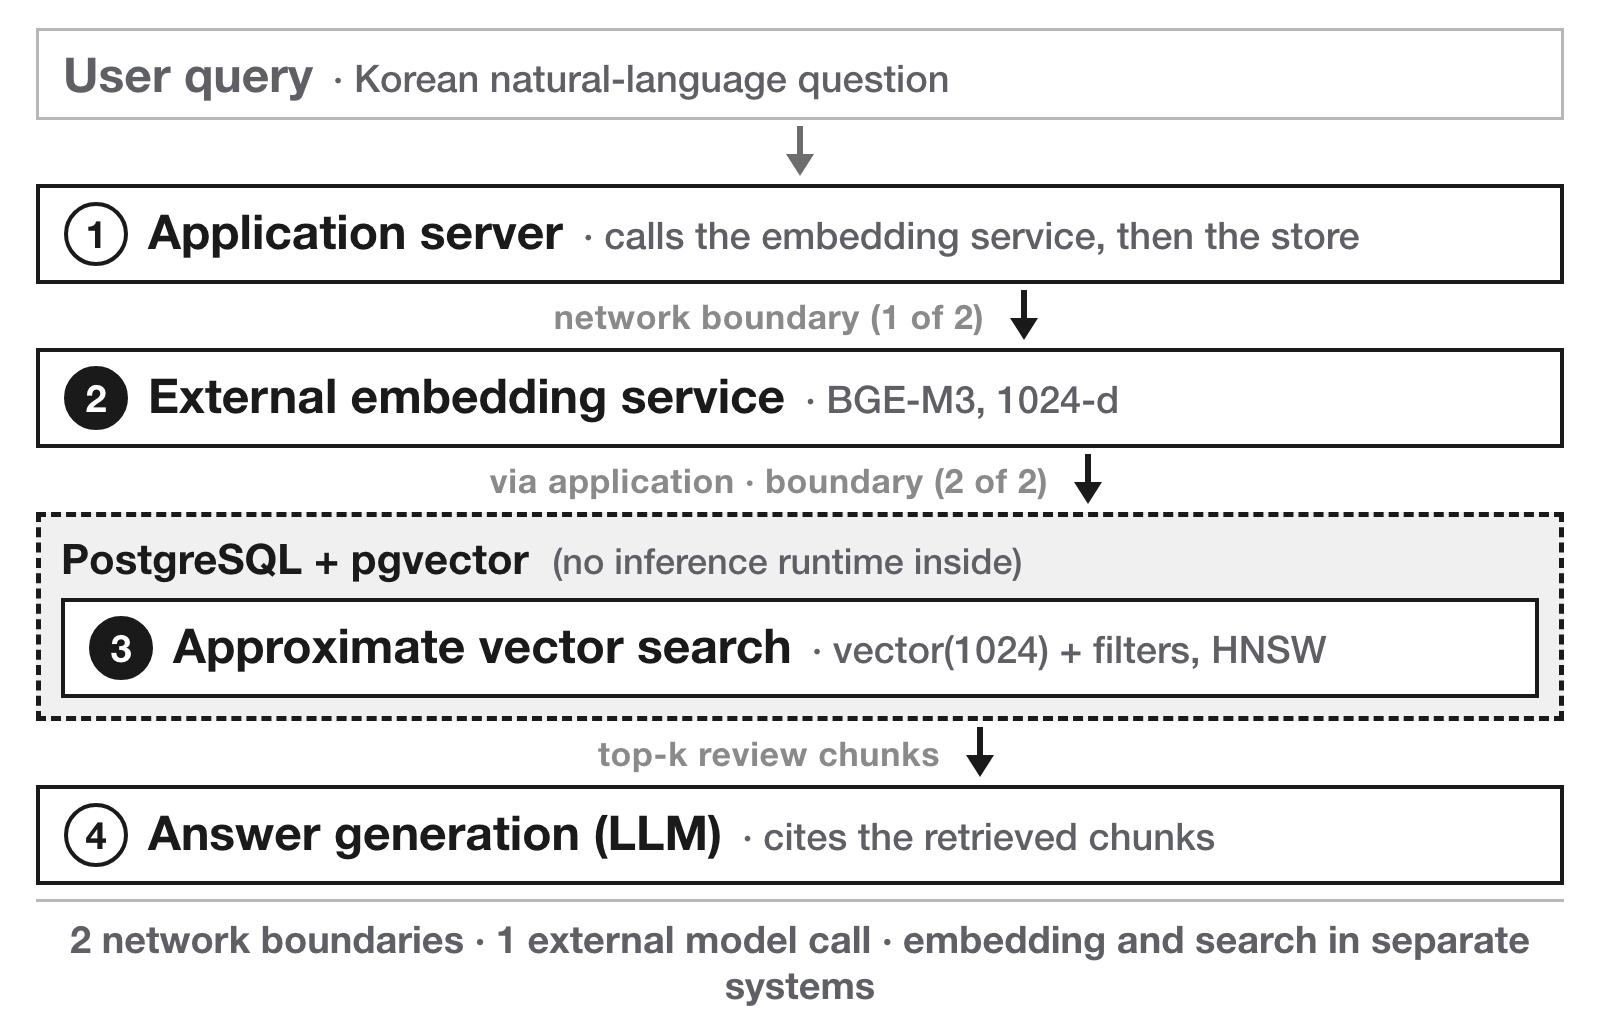
\includegraphics[width=\linewidth]{../../figures/paper-fig2-arch-pgvector.png}\par
  \vspace{5pt}
  {\fontsize{8}{9.6}\selectfont Fig. 2. PostgreSQL-based system architecture}
\end{minipage}
\end{figure*}

As a result, the end-to-end difference alone does not reveal which factor caused the change. When quality drops, it cannot be told apart whether the store or the model is at fault, and when nothing changes, it cannot be known whether the two factors cancelled each other out. In either case the conclusion cannot be carried over as is to an environment with a different instance class or model-size constraint.

This paper inserts an intermediate condition, the bridge condition, that loads the target store with the embeddings the source system has already produced, and thereby splits one comparison in which the two factors are entangled into two comparisons that each differ in one factor at a time. We apply the proposed method to a Korean review-analysis service migrated from a PostgreSQL vector extension to a converged database that supports in-database embedding, and measure it on 1,347 review chunks from the production corpus and 43 fixed queries. This paper does not judge which product is superior, and the latency figures reflect the measurement environment rather than the products.

% ======================================================================
% 2. Proposed Method
% ======================================================================
\pgsec{2. Proposed Method}

\pgsubsec{2.1 System Architecture}

The target system retrieves Korean product reviews and generates answers that cite the retrieved evidence. Both architectures operate in four stages: query input, query embedding, vector search, and answer generation. Retrieval is a hybrid scheme that combines vector similarity with metadata filters and source-based prioritization, and this rule and its parameters were kept identical across the three conditions. Because both are expressed as a single SQL statement, the store and the embedding placement can be swapped while the application logic is left as it is.

Fig. 1 shows the Oracle-based architecture. The application sends a single SQL statement carrying the query string (step 1), and the database converts the query into a 384-dimensional vector with its built-in ONNX inference runtime (step 2) and then, within the same SQL statement, performs an exact search over the VECTOR column together with metadata filtering (step 3). The language model cites the returned top-$k$ chunks to generate an answer (step 4).

Fig. 2 shows the PostgreSQL-based architecture. The application calls an external embedding service to convert the query into a 1024-dimensional vector (step 2) and then requests the search with that vector as an argument (step 3). The store explores candidates with an HNSW approximate index and applies the same filters, and the remaining steps are as in Fig. 1.

The two architectures differ in two things at once, the store and the embedding placement. One is which engine holds the vectors and with what indexing method, and the other is whether the embedding is computed outside or inside the database. An end-to-end comparison alone cannot tell which of the two produced the difference. The next two subsections summarize the characteristics of each architecture from these two viewpoints, and Section 3 presents a way to separate them.

\pgsubsec{2.2 Characteristics of the Oracle-Based Architecture}

First, it provides a native VECTOR type and a built-in ONNX inference runtime, so embedding and search are combined into a single SQL statement [3]. Second, it performs an exact search that compares every vector, without an approximate index that narrows candidates in advance, so no correct result is missed because of the index. Third, the network boundary is reduced to one, and because the query and the retrieved results stay inside the database, controls such as encryption and auditing apply to the entire retrieval path. Fourth, a built-in model follows the model-file size limit the database allows, and in this environment the largest multilingual model within that limit was multilingual-e5-small (384 dimensions) [4].

\pgsubsec{2.3 Characteristics of the PostgreSQL-Based Architecture}

First, it provides vector search through an extension module (pgvector) and contains no inference runtime [5]. The embedding model can be chosen separately from the store, so there is no size constraint, and this architecture uses the 1024-dimensional BGE-M3 [6]. Second, it uses an HNSW approximate index that narrows candidates as it searches, so search time grows gently as the data grows, at the cost of missing some correct results [7]. Third, because the embedding is computed externally, the query text leaves the store boundary and one more network round trip is required.

% ======================================================================
% 3. Performance Evaluation
% ======================================================================
\pgsec{3. Performance Evaluation}

\pgsubsec{3.1 Experimental Setup}

% Table 1 (experimental conditions, section 3.1)
\begin{table}[t]
\centering
{\fontsize{8}{9.6}\selectfont Table 1. Experimental conditions}
\vspace{4pt}

\fontsize{6.9}{8.1}\selectfont
\setlength{\tabcolsep}{2pt}
\renewcommand{\arraystretch}{0.95}
\begin{tabular}{@{}l>{\raggedright\arraybackslash}p{1.85cm}>{\raggedright\arraybackslash}p{1.85cm}>{\raggedright\arraybackslash}p{1.85cm}@{}}
\toprule
 & A (baseline) & B (bridge) & C (migrated) \\
\midrule
Store & PostgreSQL + pgvector & Oracle 26ai & Oracle 26ai \\
Embedding model & BGE-M3 (1024) & BGE-M3 (1024) & e5-small (384) \\
Placement & external & external & in-database \\
Vector search & HNSW approx. & exact & exact \\
\bottomrule
\end{tabular}

\vspace{4pt}
{\fontsize{6.9}{8.1}\selectfont A$\rightarrow$B changes only the store factor, and B$\rightarrow$C only the placement factor. e5-small denotes multilingual-e5-small.}
\end{table}

In this experiment we denote a retrieval configuration by the triple $(S, E, P)$, where $S$ is the store, $E$ is the embedding model, and $P$ is where the embedding is executed. Comparing the two architectures of Section 2 as they are amounts to comparing $(S_0, E_0, \text{external})$ with $(S_1, E_1, \text{in-database})$; all three coordinates differ, so the contribution of each factor cannot be separated. We therefore add $(S_1, E_0, \text{external})$, a bridge condition that uses the target store but is loaded with the vectors the source system produced, and the three conditions are summarized in Table 1. The bridge condition needs no recomputation of the vectors. Because the columns in production are left as they are and only one more vector column is created and filled, its preparation cost is a single bulk load and the running service is not touched.

In condition C, however, moving the placement also changes the model, because the file-size limit of Section 2.2 makes it impossible to host the source model inside the database. Choosing in-database placement means accepting that limit as well, so this coupling was left in place on purpose. Separating the two would require one more condition, $(S_1, E_1, \text{external})$, which runs the smaller model outside the database, and we leave this to future work.

The corpus consists of 1,347 review chunks from a single product domain of the production service, loaded identically into both stores after verifying in advance that the chunk identifiers correspond one to one. The query set was fixed at 43 Korean queries, 13 drawn from production logs and 30 synthetic queries written so as to cover evenly the evaluation aspects and purchase-journey stages the service handles.

Three metrics are measured. The first is the agreement of the retrieved results: how much the top-10 results the two conditions return for the same query overlap (Jaccard), how similar their rankings are (Spearman rank correlation), and, taking the exact search of the bridge condition as ground truth, how many of those the baseline recovers (Recall@10). The second is the relevance of the retrieved evidence: a large language model scores the top-5 chunks on a 0--2 scale [8], and 215 judgments per condition are averaged per query and then compared in pairs across the same queries. The third is the actual time taken to process a single query.

The target database ran on the lowest-tier free instance (Always Free, 2 GB RAM) and the external embedding service on a local laptop (Apple M5 Pro). Confidence intervals were obtained by bootstrap resampling of the measurements 10,000 times.

\pgsubsec{3.2 Experimental Results}

% Table 2 (results, section 3.2)
\begin{table}[t]
\centering
{\fontsize{8}{9.6}\selectfont Table 2. Results by factor}
\vspace{4pt}

\fontsize{6.9}{8.1}\selectfont
\setlength{\tabcolsep}{2pt}
\begin{tabular}{@{}lcc@{}}
\toprule
Metric & A $\rightarrow$ B (store) & B $\rightarrow$ C (placement) \\
\midrule
Top-10 Jaccard [95\% CI] & 0.971 [0.946, 0.992] & 0.175 [0.133, 0.221] \\
Spearman rank correlation & 0.958 & --- \\
Recall@10 (vs. exact search) & 0.984 & --- \\
Relevance score (0--2) & 1.228 $\rightarrow$ 1.270 & 1.270 $\rightarrow$ 1.014 \\
Paired difference [95\% CI] & $-$0.042 [$-$0.172, 0.084] & 0.256 [0.098, 0.423] \\
Significance / effect size $d_z$ & $p = 0.523$ / $-$0.098 & $p = 0.003$ / 0.473 \\
Mean search latency (ms) & 150.2 $\rightarrow$ 110.0 & 110.0 $\rightarrow$ 947.0 \\
External calls / boundaries & 1$\rightarrow$1 / 2$\rightarrow$2 & 1$\rightarrow$0 / 2$\rightarrow$1 \\
\bottomrule
\end{tabular}

\vspace{4pt}
{\fontsize{6.9}{8.1}\selectfont Relevance is the per-query mean over the 43 queries (215 judgments per condition), and $p$ values are from a paired $t$-test.}
\end{table}

The measurements by factor are summarized in Table 2.

Looking first at ranking agreement, the two stores loaded with identical vectors returned exactly the same top-10 set for 37 of the 43 queries, and even the minimum was 0.667. The results the baseline missed because of its approximate index amount to about 1.6\%.

For the store factor, the paired difference in relevance scores across the same queries was not statistically significant and the effect size was negligible ($t(42) = -0.643$). A Wilcoxon test on the 28 queries that remain after excluding those with identical scores leads to the same conclusion ($p = 0.908$).

Since ``no difference'' is itself our claim, we did not rely only on a non-significant $p$ value but tested equivalence separately [9]. Two one-sided tests examining whether the difference falls within $\pm$0.15 points gave $p = 0.052$: the lower bound of the confidence interval, $-$0.172, falls outside this range, so the significance level was not met. We therefore report not that equivalence has been established but that no effect was detected and that its magnitude is bounded to a small range. Since the direction in which the interval extends is the one where the target store scores higher, there is no basis for concluding that substituting the store degraded quality.

By contrast, between B and C, which share the same store and the same search method, the results differ greatly. The top-10 Jaccard falls to 0.175, so mostly different evidence is retrieved for the same query, and the relevance score decreases from 1.270 to 1.014. This difference is significant with a medium effect size ($t(42) = 3.104$), and a Wilcoxon test on the 38 queries that remain after excluding those with identical scores leads to the same conclusion ($p = 0.006$). Because no store effect was detected in the change from A to B, virtually all of the end-to-end quality change is due to the placement factor and the model-capacity limit that comes with it. Had only an end-to-end comparison been performed, the roughly 20\% drop in relevance would have been blamed on the store, and reverting the store, the remedy that follows from that diagnosis, would not bring the quality back.

For search latency, the ratio of C to B was 8.27 times at the median (Wilcoxon $p < 0.001$). The increase in C is not a property of in-database embedding itself but a consequence of running inference on a free-tier instance, so it cannot be generalized to higher-tier hardware. Since A and B produce the same vectors with the same external service, the query embedding time was measured once and applied to both conditions, and the latency difference between them therefore reflects only the store search time.

Finally, because 30 of the 43 queries are synthetic, we checked whether they behave differently from the 13 real queries. Relevance scores were systematically lower on the synthetic subset (A: 1.147 vs. 1.415, $p = 0.045$; C: 0.880 vs. 1.323, $p = 0.007$; Mann--Whitney), so the absolute level of relevance must not be read as service quality. In contrast, ranking agreement, the basis on which the cause is attributed, showed no significant difference between the two subsets ($p = 0.441$, $p = 0.570$). Absolute scores depend on where the queries come from, but the conclusion about the cause is the same on both.

% ======================================================================
% 4. Conclusion
% ======================================================================
\pgsec{4. Conclusion}

Adding a single bridge condition makes it possible to split an end-to-end comparison into two single-factor comparisons. Applied to a Korean review RAG service in production, no effect of the store factor was detected, and the entire observed change originated from the placement factor. Changing the placement is a trade in governance rather than in performance. In exchange for keeping the query and the review text inside the database boundary, one has to accept the capacity limit of the model and the inference performance of the database tier. Therefore, if governance of the stored data is the only goal, replacing the store alone is enough, and if the query path must also stay inside the boundary, one should first confirm that the largest model that can be hosted is sufficient for that domain. The bridge condition makes that confirmation possible before the migration is carried out.

The limitations are as follows. The study targets a single Korean corpus of 1,347 chunks, human assessors were not involved in the relevance scoring, and the measurements were taken on an entry-level instance. In addition, as stated in Section 3.1, placement and model capacity are coupled by construction, and the result for the store factor does not establish equivalence.

% ======================================================================
% NOTE: Conflict of Interest is camera-ready only.
% Author Guidelines §9 "Camera-ready Only Sections" lists Author Information,
% Acknowledgement and the Conflict of Interest statement as sections to be
% included "only after acceptance", so the review version omits it.
% The statement is retained in pygeek2026-en-camera.tex.
% ======================================================================
\pgspecial{References}

{\setstretch{1.0}\setlength{\parskip}{0pt}\fontsize{8}{9.2}\selectfont\raggedright

\noindent\hangindent=0.5cm\hangafter=1
[1] P. Lewis et al., ``Retrieval-augmented generation for knowledge-intensive NLP tasks,'' Advances in Neural Information Processing Systems, vol. 33, pp. 9459-9474, 2020.
\par\vspace{0pt}

\noindent\hangindent=0.5cm\hangafter=1
[2] Y. Gao et al., ``Retrieval-augmented generation for large language models: A survey,'' arXiv preprint arXiv:2312.10997, 2023.
\par\vspace{0pt}

\noindent\hangindent=0.5cm\hangafter=1
[3] Oracle, ``Oracle AI Vector Search User's Guide,'' Oracle AI Database 26ai documentation, Available: \url{https://docs.oracle.com/en/database/oracle/oracle-database/26/vecse/}, 2026, [Accessed: Aug. 8, 2026].
\par\vspace{0pt}

\noindent\hangindent=0.5cm\hangafter=1
[4] L. Wang, N. Yang, X. Huang, L. Yang, R. Majumder, and F. Wei, ``Multilingual E5 text embeddings: A technical report,'' arXiv preprint arXiv:2402.05672, 2024.
\par\vspace{0pt}

\noindent\hangindent=0.5cm\hangafter=1
[5] pgvector, ``pgvector: Open-source vector similarity search for Postgres,'' GitHub repository, Available: \url{https://github.com/pgvector/pgvector}, 2026, [Accessed: Aug. 8, 2026].
\par\vspace{0pt}

\noindent\hangindent=0.5cm\hangafter=1
[6] J. Chen, S. Xiao, P. Zhang, K. Luo, D. Lian, and Z. Liu, ``M3-Embedding: Multi-linguality, multi-functionality, multi-granularity text embeddings through self-knowledge distillation,'' Findings of the Association for Computational Linguistics: ACL 2024, Bangkok, Thailand, pp. 2318-2335, \url{https://doi.org/10.18653/v1/2024.findings-acl.137}, Aug., 2024.
\par\vspace{0pt}

\noindent\hangindent=0.5cm\hangafter=1
[7] Y. A. Malkov and D. A. Yashunin, ``Efficient and robust approximate nearest neighbor search using hierarchical navigable small world graphs,'' IEEE Transactions on Pattern Analysis and Machine Intelligence, vol. 42, no. 4, pp. 824-836, \url{https://doi.org/10.1109/TPAMI.2018.2889473}, 2020.
\par\vspace{0pt}

\noindent\hangindent=0.5cm\hangafter=1
[8] L. Zheng et al., ``Judging LLM-as-a-Judge with MT-Bench and Chatbot Arena,'' Advances in Neural Information Processing Systems 36 (NeurIPS 2023), Datasets and Benchmarks Track, 2023.
\par\vspace{0pt}

\noindent\hangindent=0.5cm\hangafter=1
[9] D. Lakens, ``Equivalence tests: A practical primer for t tests, correlations, and meta-analyses,'' Social Psychological and Personality Science, vol. 8, no. 4, pp. 355-362, \url{https://doi.org/10.1177/1948550617697177}, 2017.
\par
}


\end{document}
